\documentclass{beamer}
\usepackage[english]{babel}
\usepackage{amsmath}
\usepackage{amsfonts}
\usepackage[utf8]{inputenc}
% Стиль презентации
\usetheme{boxes}
\begin{document}
\title{An application for dynamic object identification based on lucas-kanade algorithm}  
\author{Kostenko Dmitry}

\date{Moscow, 2013} 
% Создание заглавной страницы
\frame{\titlepage}




\begin{frame}{Traffic conjunctions}
	\frametitle{Traffic conjunctions}
	\begin{center}
		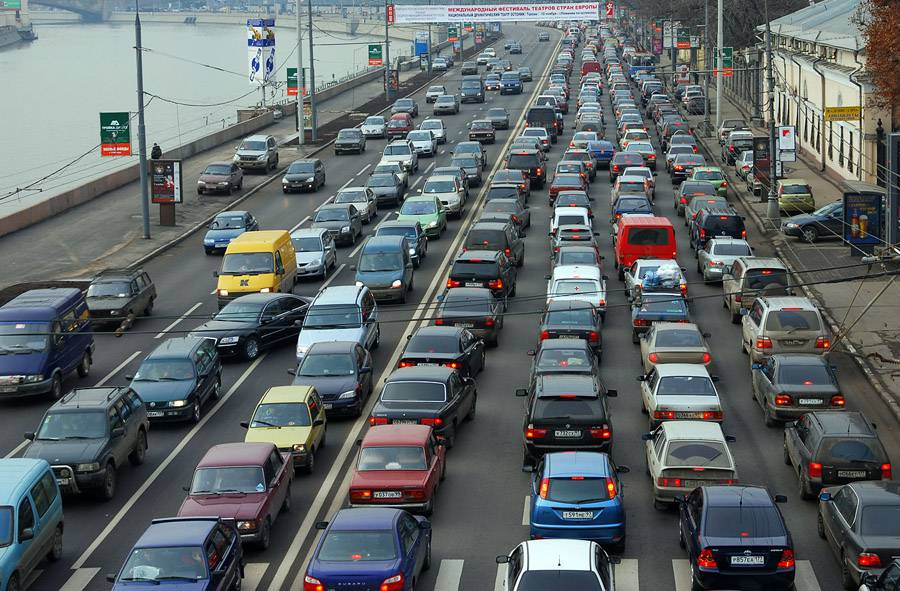
\includegraphics[width= 0.8\linewidth]{images/traffic_jam.jpg}  
	\end{center}
\end{frame}



\begin{frame}{ITS}
	\frametitle{Intelligent Transportation System}
	\begin{center}
		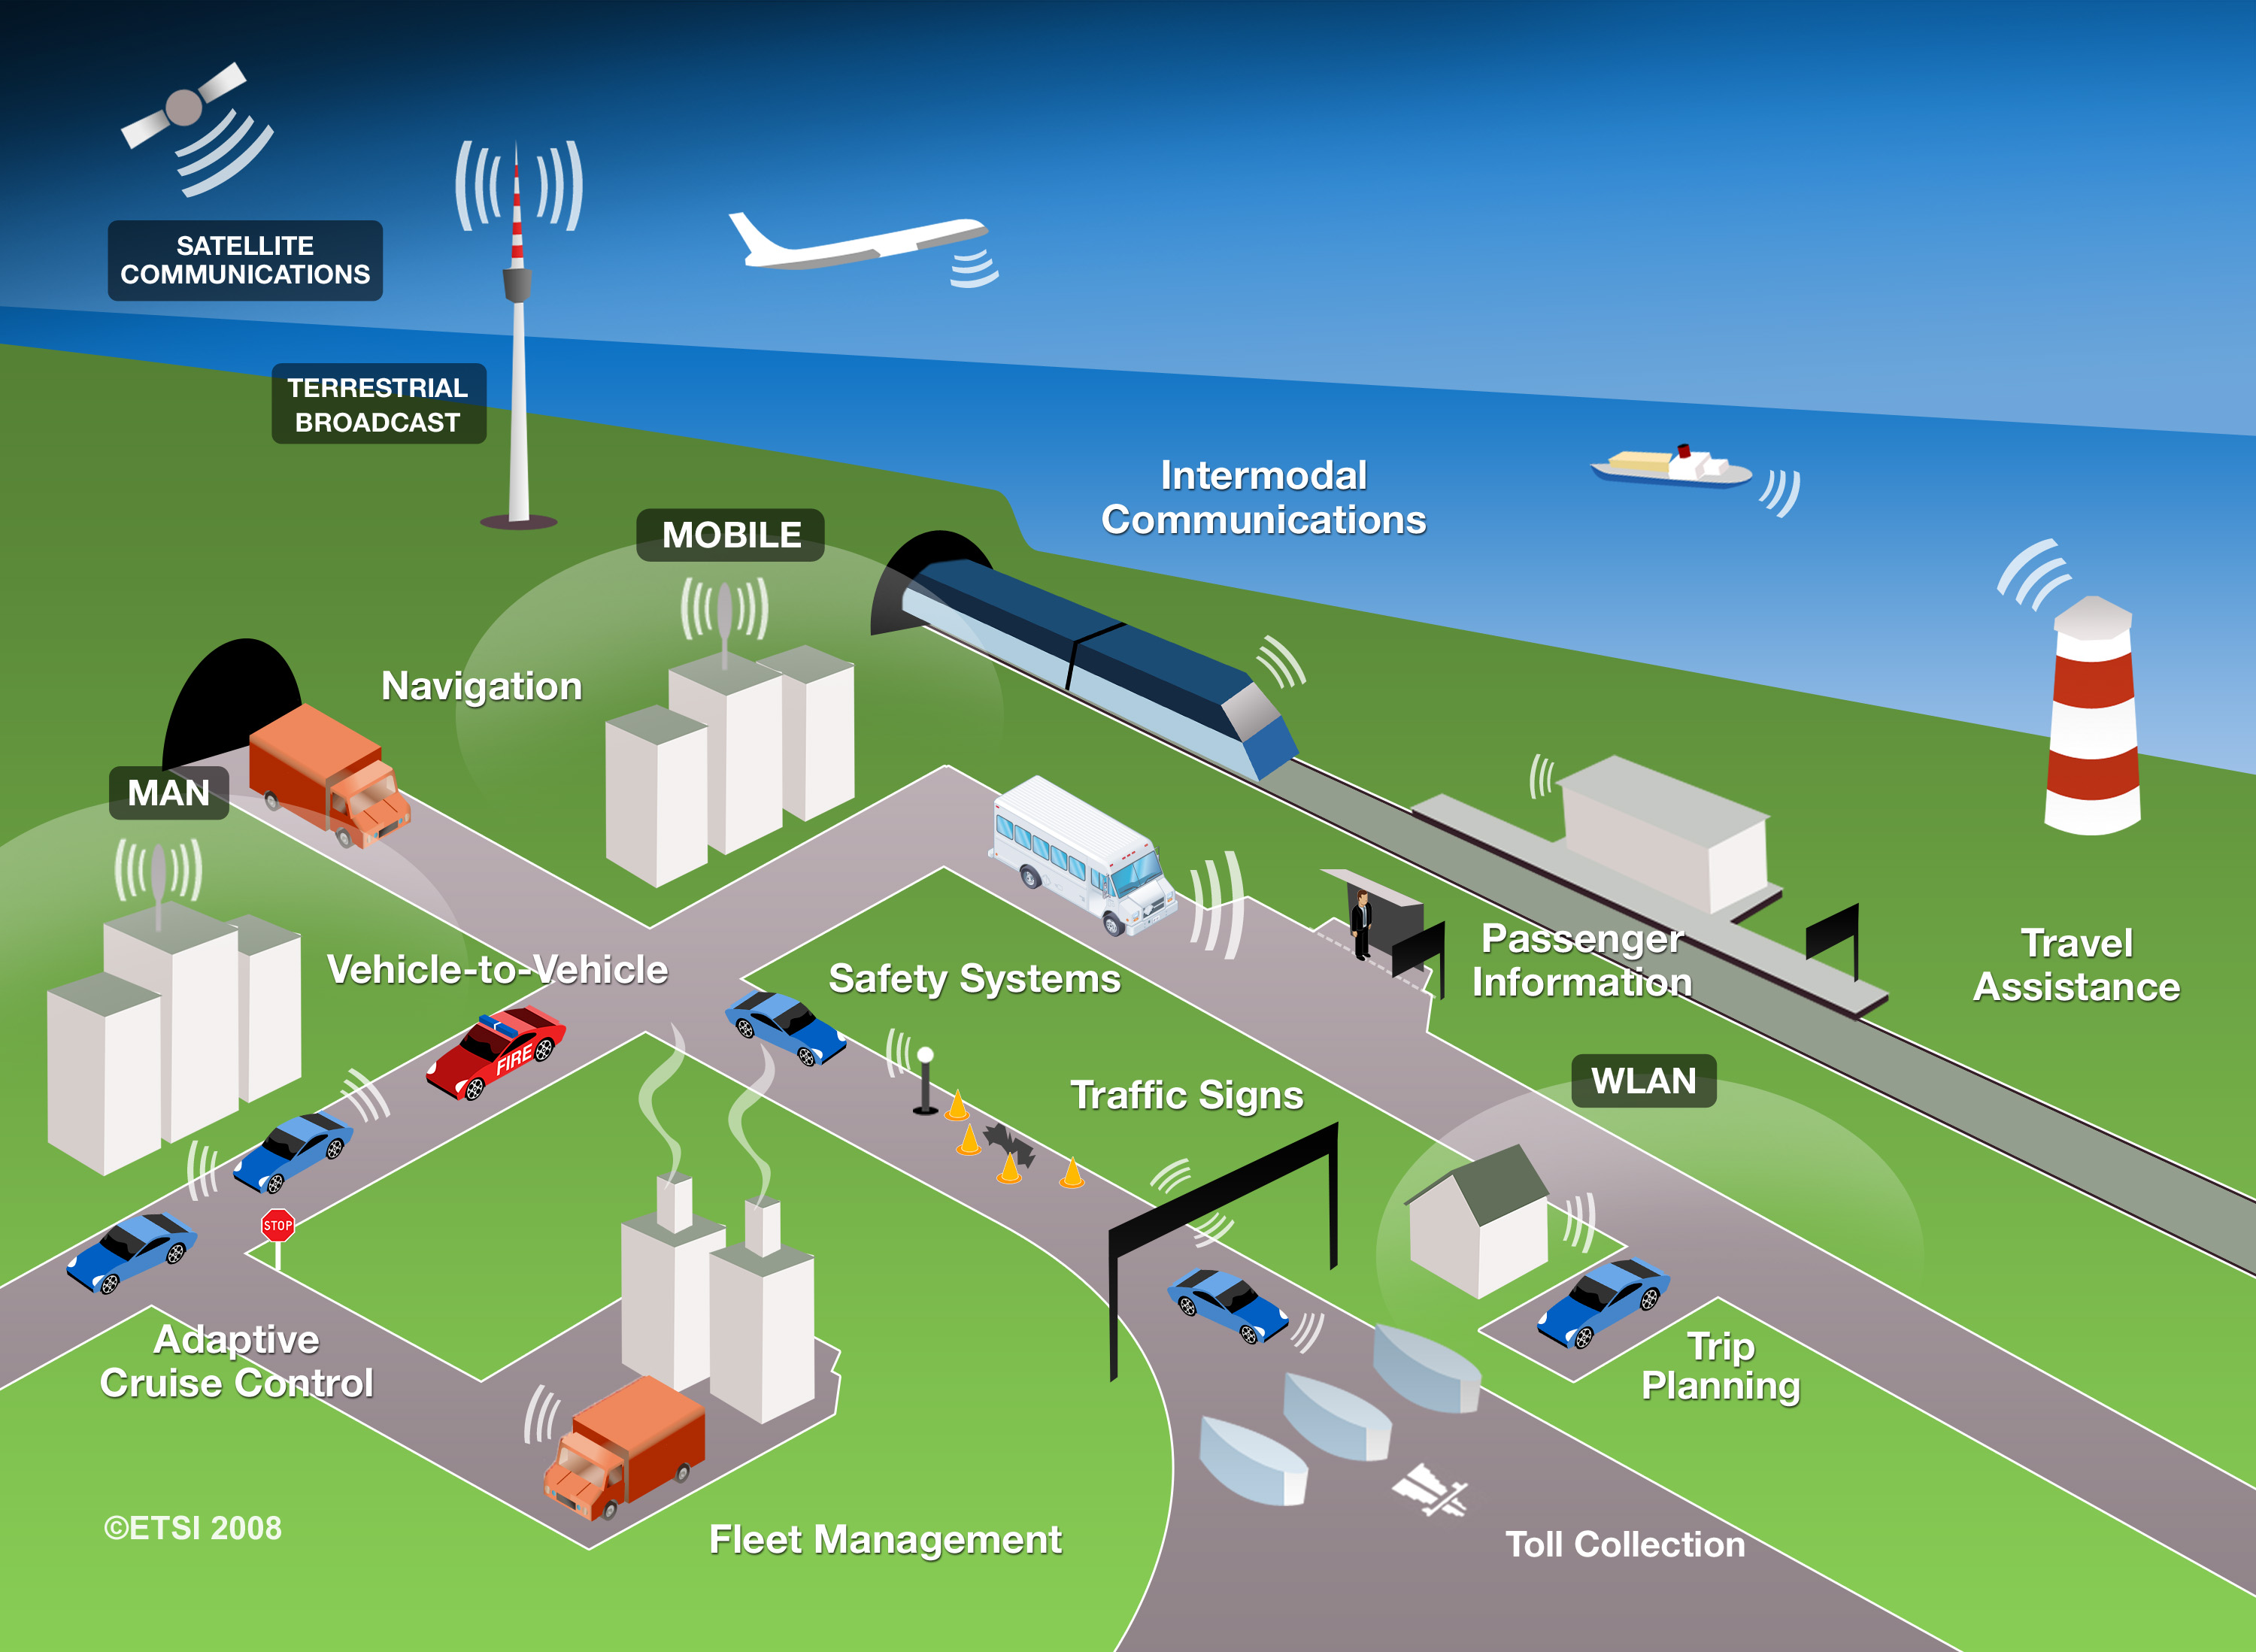
\includegraphics[width= 0.8\linewidth]{images/its.jpg}  
	\end{center}
\end{frame}


\begin{frame}{Vehicle counting}
	\frametitle{Vehicle counting}
	\begin{center}
		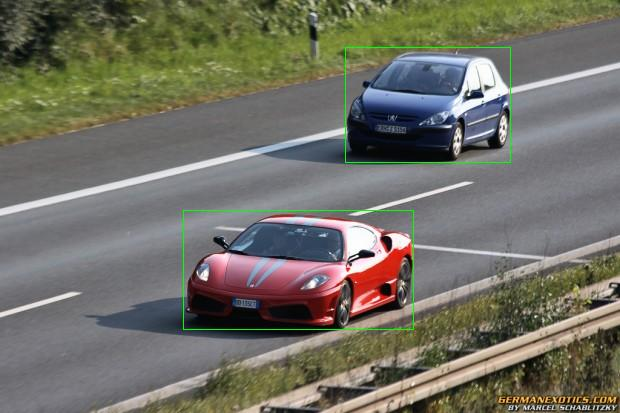
\includegraphics[width= 0.8\linewidth]{images/cars.jpg}  
	\end{center}
\end{frame}



\begin{frame}{Isolated areas}
	\frametitle{Isolated areas}
	\begin{center}
		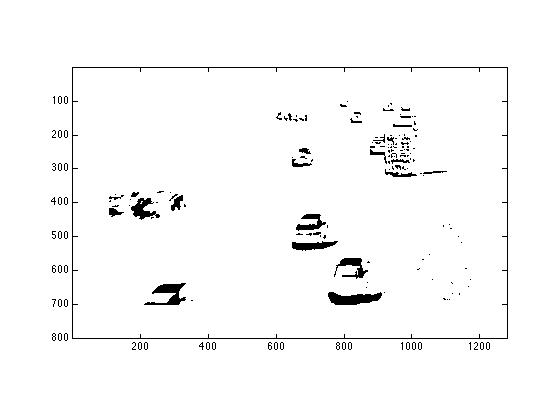
\includegraphics[width= 0.8\linewidth]{images/isolated_areas.jpg}  
	\end{center}
\end{frame}


\begin{frame}{From short-term to long-term}
	\frametitle{From short-term to long-term}
	\begin{figure}[b]
		\centering
		
\includegraphics[width=0.2\textwidth]{images/frame1.png}
		
\includegraphics[width=0.2\textwidth]{images/frame2.png}
		
\includegraphics[width=0.2\textwidth]{images/frame3.png}
		
\includegraphics[width=0.2\textwidth]{images/frame4.png}
		\label{figur}\caption{equation...}
	\end{figure}
\end{frame}


\end{document}